\chapter{Results and Interpretation}
\label{chap:results}
\shorttitle{\nameref{chap:results}}

This chapter analyzes whether the \ac{ros2} driver for the e-puck2 physical robot and the \ac{ros2} universal driver provide expected behavior. The analysis will be shown through three pillars:
\begin{itemize}
    \item Verify whether the e-puck2 physical and simulated robots have a similar behavior with the same controller.
    \item Verify whether simulated e-puck2 and Khepera IV robots have a similar behavior with the same controller.
    \item Verify whether the \ac{ros2} universal driver works properly with the other robots such as TIAGo++ and TurtleBot3 Burger.
\end{itemize}

% This chapter quantifies the difference between the simulated e-puck2 and the physical robot's performance, also including the Khepera IV simulated robot, showing that the \ac{ros2} interface is appropriately implemented. 
% The impact of generalized \ac{ros2} will also be described. 

\section{Comparison of Physical and Simulated E-puck2}

In this section, we want to verify whether the \ac{ros2} interface is the for the physical and simulated e-puck2 robots.
In that respect, endpoints of the \ac{ros2} interface of the physical and the simulated e-puck2 robots will be individually compared.
The difference of the \ac{ros2} interfaces will then be quantified with \ac{ros2} navigation and mapping controllers.

\subsection{\ac{ros2} Interface Endpoints Comparison}

% First, the readings from the sensors need to be compared. Most of the sensors of the e-puck2 simulated robot are calibrated before this project has taken place.
% Therefore, a quick visual inspection was enough to verify that the sensors have the desired output.
The \ac{ros2} interfaces for physical and simulated robots are very similar, image-related topics being the only difference.
The physical e-puck2 robot advertises \texttt{/image\_raw/compressed} topic of type \texttt{sensor\_msgs/CompressedImage} and the robot uses it to transfer compressed images over the network.

\subsection{Camera Performance Comparison}
This benchmark has to compare different \ac{ros2} camera node implementations on the physical e-puck2 robot, at which resolution and \ac{fps} it can operate.
The analysis aims to determine a suitable way to transport the images from Raspberry Pi Zero W and identify bottlenecks.

In terms of compression, the images are transported as raw, \ac{jpeg} compressed and as a Theora compressed video stream\footnote{Description of the Theora technology is available at the official website - \url{https://www.theora.org/}}.
In terms of color encoding, \ac{rgb} and \acs{yuv} are tested.
And in terms of nodes separation, the testing node was located on-board or on workstation while communicating to the Raspberry Pi Zero W over Wi-Fi.

In the Table \ref{tab:results:camera_perf}, performances are measured in \ac{fps} and the measurements are given for different camera implementations.

\begin{table}[H]
    \begin{adjustwidth}{-1.5in}{-1.5in} 
    \centering
    \begin{tabular}{|l|c|c|c|}
        \hline
         & 32x24 [\ac{fps} ($ \sigma $)] & 160x120 [\ac{fps} ($ \sigma $)] & 640x480 [\ac{fps} ($ \sigma $)] \\
         \hline
         RAW over Wi-Fi & 13.95 (0.009s) & 10.08 (0.013s) & 1.62 (0.096s) \\
         \hline
         RAW on-board & X & X & 3.80 (0.064s) \\
        \hline
        JPEG over Wi-Fi & X & X & 2.97 (0.105s) \\
        \hline
        JPEG over Wi-Fi with white-noise & X & X & 0.95 (0.998s) \\
        \hline
        JPEG on-board & X & X & 2.10 (0.016s) \\
        \hline
        RAW on-board without YUV42RGB & X & X & 5.04 (0.037s) \\
        \hline
        Theora over Wi-Fi & X & X & 1.25 (0.054s) \\
        \hline
        Theora on-board & X & X & 1.03 (0.026s) \\
        \hline
        Custom over Wi-Fi & 10.079 (0.073s) & 9.981 (0.076s) & 9.904 (0.079s) \\
        \hline
    \end{tabular}
    \end{adjustwidth}
    
    \caption{\ac{fps} measurements in different configurations within \ac{ros2} environment}
    \label{tab:results:camera_perf}
\end{table}

Please note that the experiments have been done under the following conditions:
\begin{itemize}
    \item Package \texttt{v4l2\_camera} is used to read and transport images. The package works as following:
        \begin{itemize}
            \item the images are read directly from memory using \texttt{mmap()} in YUV422\_YUY2 format (native camera format),
            \item the images are converted to \ac{rgb} color encoding using \texttt{cv\_bridge} package
            \item the images are transported using \texttt{image\_transport}, \texttt{image\_transport\_plugins} (equipped with \texttt{compressed\_image\_transport} and \texttt{theora\_image\_transport}) with default configuration,
            \item the package is alternated to accommodate image resize for this experiment and the image resizing is done just before YUV422\_YUY2 to \ac{rgb} conversion
            \item the package is implemented in C++ with attention to memory management (the image is cloned only when necessary).
        \end{itemize}
    \item Camera is configured to 15 \ac{fps}.
    \item \ac{fps} measurements are done using \texttt{ros2 topic hz}.
    \item The Wi-Fi network performance measurements are performed using \texttt{iperf3} and the following results acquired:
        \begin{itemize}
            \item 16.4 Mbits/sec for transfer from \ac{pc} to Raspberry Pi Zero W and
            \item 13.8 Mbits/sec for transfer from Raspberry Pi Zero W to \ac{pc}.
        \end{itemize}
    \item White noise is simulated by putting finger on the camera.
    The assumption is that the low light condition produces a lot of white noise. 
\end{itemize}

The measured data transfer between the Raspberry Pi Zero W and the \ac{pc} during the publishing of the raw images is 12.8Mb/s.
Since every image is sent in \ac{rgb} format, that means 7Mbits per image ($ 8 \times \frac{ 3 \times 640 \times 480 }{1024 \times 1024}$), or at 1.62 \ac{fps}, it is 11.4Mbits/s.
Therefore, by sending raw images, we expected to encounter the limitations of the Wi-Fi network.

In all other methods that require compression (\ac{jpeg} or Theora), the \ac{cpu} on Raspberry Pi Zero W was hitting 100\% of workload.
Therefore, in those cases, the \ac{cpu} is the bottleneck.

It may look strange that a slightly higher \ac{fps} is achieved with the images that are transferred over the network (``\ac{jpeg} over Wi-Fi'') than the images transferred locally (``\ac{jpeg} on-board''). 
It is worth noting that the Raspberry Pi Zero W has a relatively slow \ac{cpu} and that the tool used to measure performance has to allocate a certain amount of \ac{cpu} time.
Since the network is not the bottleneck here, but \ac{cpu}, the effect of another process using the \ac{cpu} is noticeable.

\begin{figure}[H]
\centering
\begin{subfigure}{.8\textwidth}
  \centering
  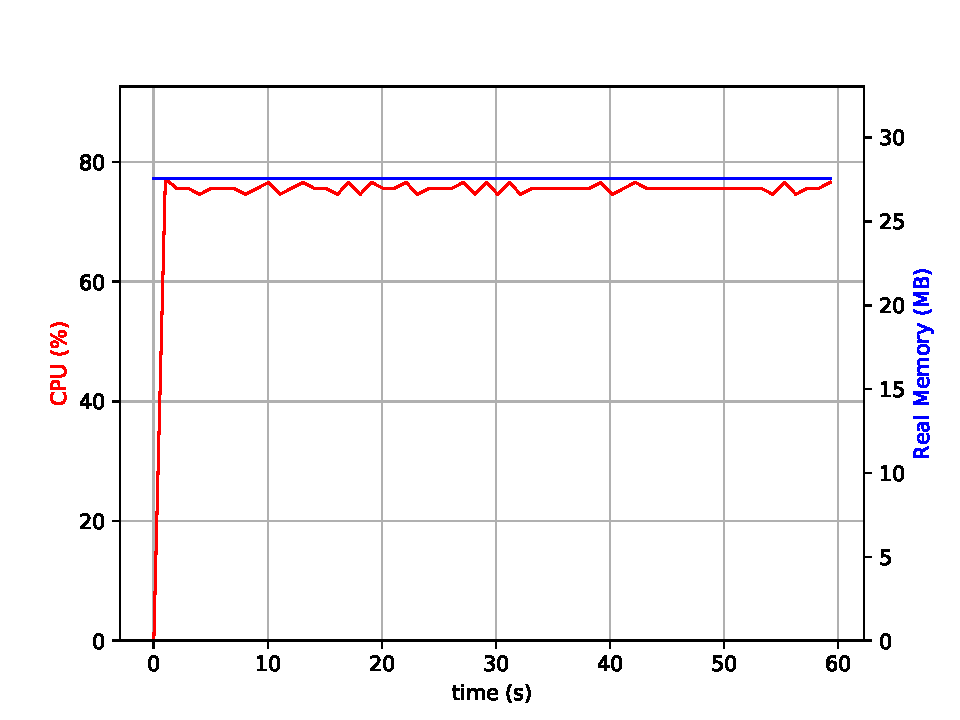
\includegraphics[width=\linewidth]{results/figures/camera_raw_cpu}
  \caption{\ac{cpu} usage while publishing raw \ac{rgb} images}
  \label{fig:results:camera_load:raw_cpu}
\end{subfigure}
\begin{subfigure}{.8\textwidth}
  \centering
  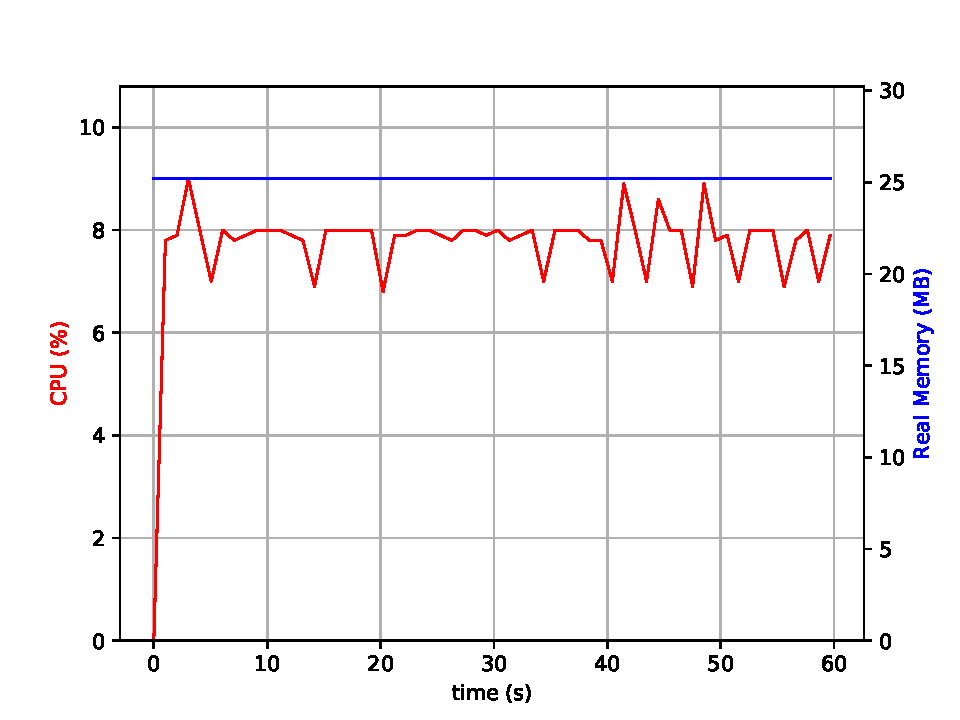
\includegraphics[width=\linewidth]{results/figures/camera_jpeg_gpu.pdf}
  \caption{\ac{cpu} usage while publishing compressed (on the \ac{gpu}) \ac{jpeg} images}
  \label{fig:results:camera_load:jpeg_gpu}
\end{subfigure}
\caption[Comparison of \ac{cpu} usage for two transfer modes, raw \ac{rgb} and \ac{jpeg} compressed on \ac{gpu}]{Comparison of \ac{cpu} usage for two transfer modes, raw \ac{rgb} (named as ``RAW over Wi-Fi" in Table \ref{tab:results:camera_perf}) and \ac{jpeg} compressed on \ac{gpu} (named as ``Custom over Wi-Fi" in Table \ref{tab:results:camera_perf})}
\label{fig:results:camera_load}
\end{figure}

To improve \ac{jpeg} compression performance and effectively increase the \ac{fps}, the compression is offloaded to \ac{gpu}.
Comparison of \ac{jpeg} image compression performed on \ac{cpu} and \ac{gpu} is depicted in Figure \ref{fig:results:camera_load}.
It shows that even though there is no compression involved, just image publishing, the images are too large for Raspberry Pi Zero W to be transmitted efficiently, and the process allocates a lot of \ac{cpu} time.
In contrast, there the images compressed with \ac{gpu} are the small and cumbersome process of compression is offloaded to \ac{gpu}, leaving the \ac{cpu} with a minimal load.

\subsection{Performance Comparison in Mapping}
In Section \ref{sec:demos:mapping}, a custom \ac{ros2} node for mapping is described. Here, it will be used by the e-puck2 physical and simulated robot for performance comparison. In that purpose, a physical map is created, as well as its digital copy in Webots (see Figure \ref{fig:results:map}).

\begin{figure}[H]
\centering
\begin{subfigure}{.452\textwidth}
  \centering
  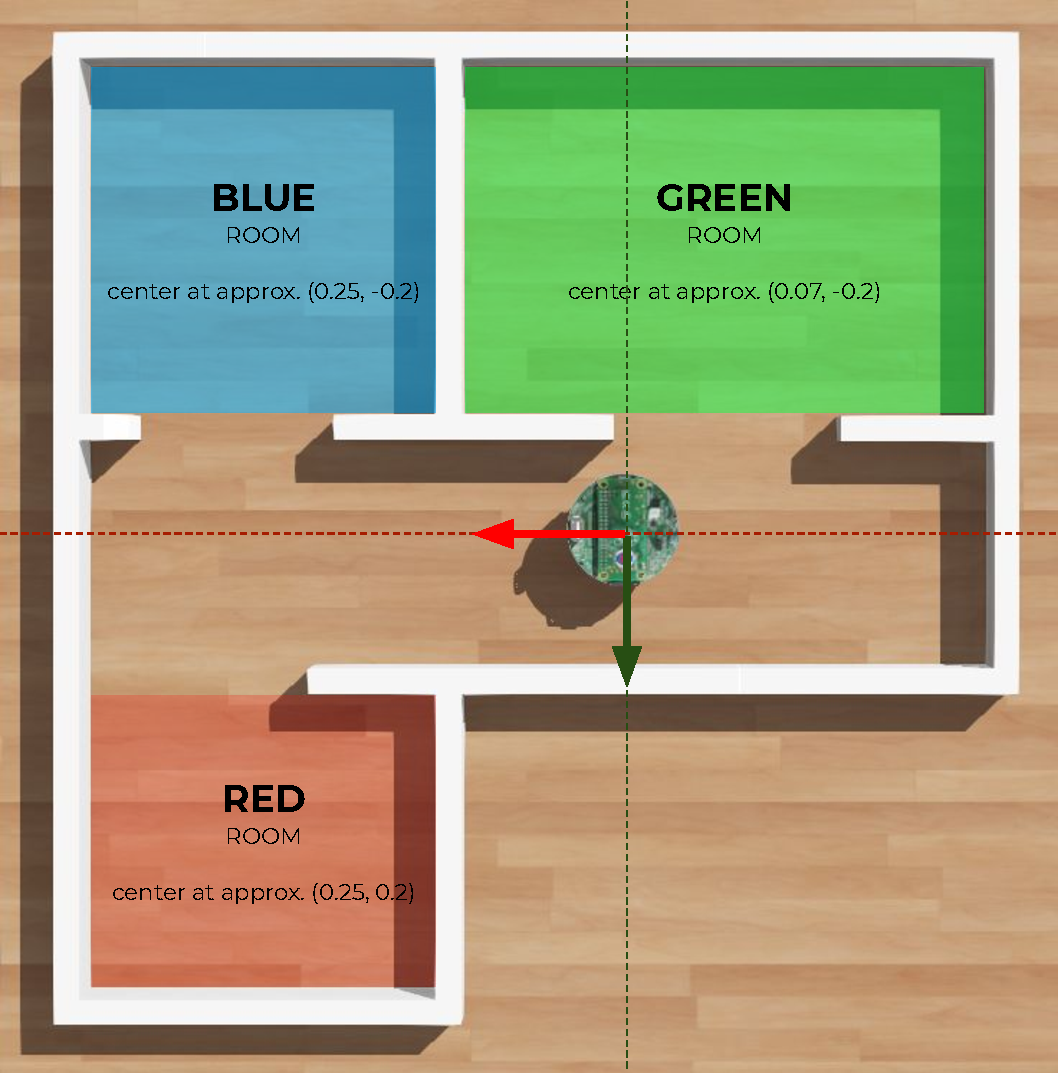
\includegraphics[width=0.97\linewidth]{results/figures/map_webots}
  \caption{Webots map}
  \label{fig:results:map:map_webots}
\end{subfigure}%
\begin{subfigure}{.448\textwidth}
  \centering
  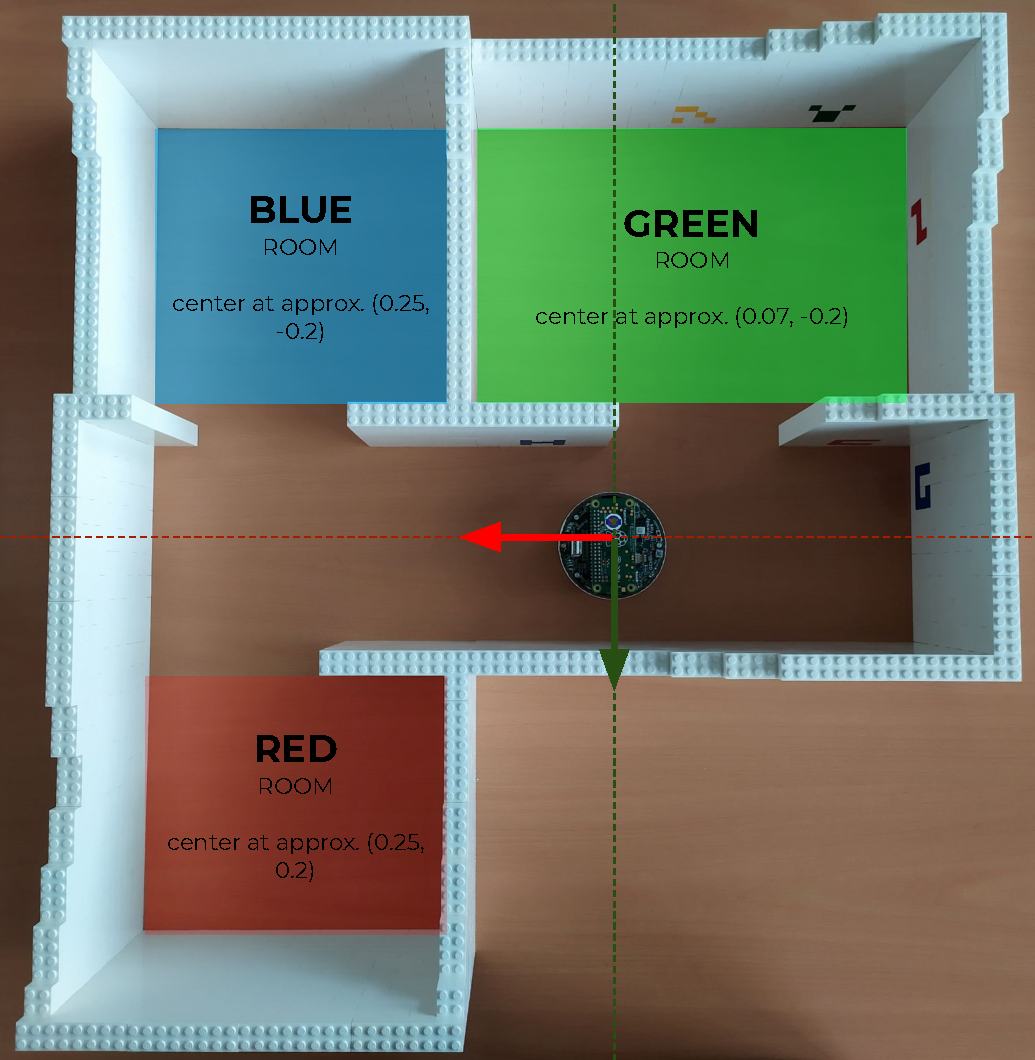
\includegraphics[width=0.97\linewidth]{results/figures/map_real_world}
  \caption{Real-world map}
  \label{fig:results:map:map_real_world}
\end{subfigure}
\caption[Webots map used for the mapping benchmark]{Webots and physical map used for the mapping benchmark with room names and coordinate systems marked}
\label{fig:results:map}
\end{figure}


To create the maps, both robots, physical and simulate, are programmed to follow the same path (see Table \ref{tab:results:list_of_poses}).
This is done to minimize the difference between the generated maps caused by differences in paths.
All maps are saved as pictures, and the comparison of the maps is shown in Figure \ref{fig:results:map_comparison}.

\begin{figure}[H]
    \centering
    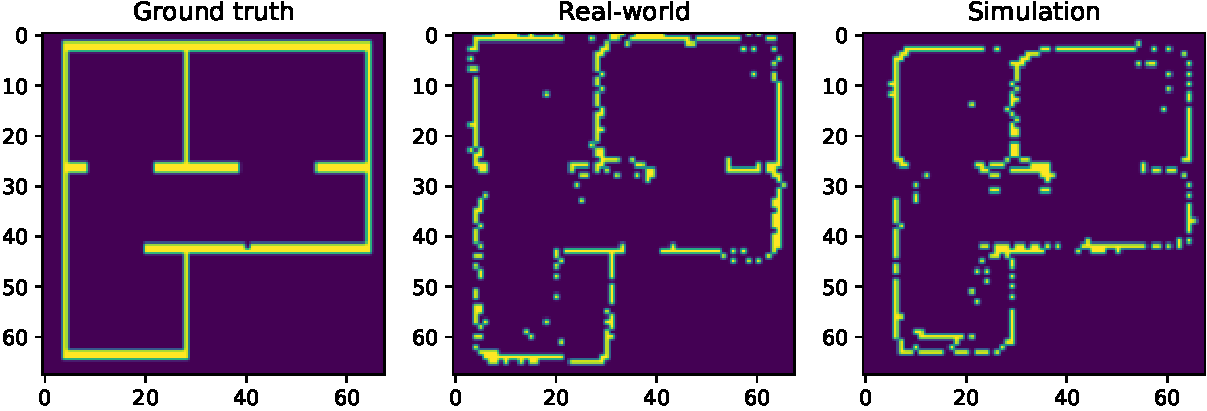
\includegraphics[width=\textwidth]{./results/figures/map_comparison.pdf}
    \caption{Comparison of the ground truth map, map created by physical robot (real-world) and map created by simulated robot (simulation)}
    \label{fig:results:map_comparison}
\end{figure}

One notices, that the quality of the maps generated in the simulation and the physical robot are similar.
However, to quantitatively compare if the quality of the maps we use \ac{iou}:

\begin{equation}
    \texttt{IoU} = \frac{\texttt{Area of Overlap}}{\texttt{Area of Union}}
\end{equation}

In which \texttt{Area of Overlap} is a number of pixels that represent a wall on both maps, while the \texttt{Area of Union} is a number of pixels represent the wall in at least one of the maps.

The \ac{iou} gives us the results shown in Table \ref{tab:results:map_iou}.

\begin{table}[H]
    \centering
    \begin{tabular}{|l|c|}
        \hline
        \textbf{Map} & \textbf{\acs{iou} with ground truth map} \\
        \hline
        Real-world \#1 & 0.2792208 \\
        \hline
        Real-world \#2 & 0.2596006 \\
        \hline
        Real-world \#3 & 0.29588607 \\
        \hline
        Simulated & 0.2993197 \\
        \hline
    \end{tabular}
    \caption{\ac{iou} of ground truth and other maps}
    \label{tab:results:map_iou}
\end{table}

The table shows that the quality of the maps is very similar.
However, to compare whether the types of errors are similar in both maps, you can check Figure \ref{fig:results:map_features}.

\begin{figure}[H]
    \centering
    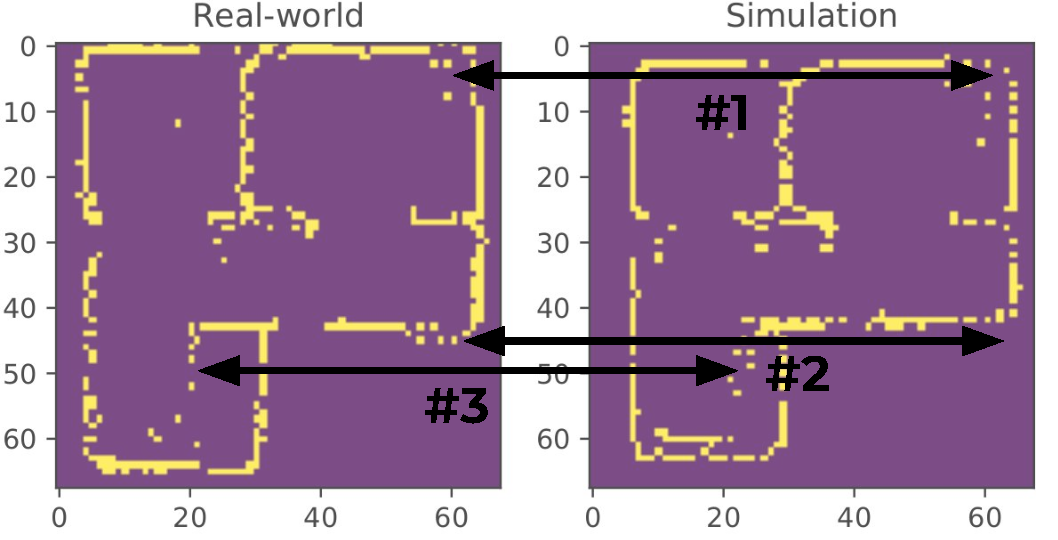
\includegraphics[width=\textwidth]{./results/figures/map_features.pdf}
    \caption{Error comparison of map obtained in simulation and real-world}
    \label{fig:results:map_features}
\end{figure}

The image shows three types of errors produced by mapping: sparse walls, rounded corners, and invisible walls.
Those three types of errors are very similar on both maps.
\begin{itemize}
    \item Error \#1: Sparse walls are a result of a low sampling rate. The robot rotates too fast to map all obstacles.
    \item Error \#2: Rounded corners are result of \ac{tof}' sensor wide \ac{fov}. The sensor doesn't measure the distance to the point, but rather it averages distance to all obstacles in its \ac{fov}.
    \item Error \#3: The invisible walls are also caused by \ac{tof}' sensor wide \ac{fov}. While the robot rotates, the distance to the obstacles gets averaged.
\end{itemize}

This experiment shows that even in more complex scenarios such as mapping, the same controller gives very similar results.
The simulated robot not only replicates the same quality of mapping but also captures the same defects. 
The observed behavior is exactly what we wanted to achieve as it proves that the same controller works correctly with the simulated and physical e-puck2 robots.

\subsection{Performance Comparison in Navigation}
\label{results:subsec:phy_navigation}

Similar to the mapping, a navigation utilizes a lot of sensors.
However, for navigation \ac{ros2} \texttt{navigation2} package is used to verify if the \ac{ros2} drivers provide satisfying results with the community packages.
The navigation is configured to use a particle filter to fix the transformation between map and odometry frame (although the weight of particle filter is much smaller in comparison to odometry).
In addition, it uses the previously obtained map in the mapping experiment.

\begin{figure}[H]
    \centering
    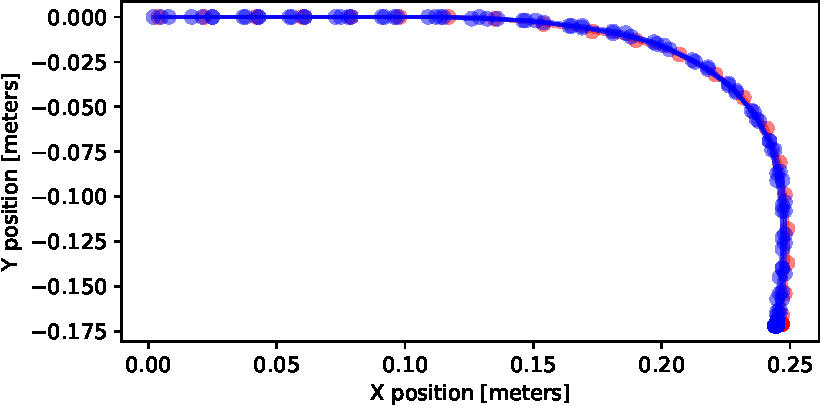
\includegraphics[width=\textwidth]{./results/figures/navigation_comparison.pdf}
    \caption{Path chosen by the simulated (red) e-puck2 robot and paths chosen by the physical (blue) e-puck2 robot}
    \label{fig:results:navigation_comparison}
\end{figure}

In Figure \ref{fig:results:navigation_comparison}, the comparison in navigation between physical and simulated e-puck2 robots is given.
The figure is obtained by sampling robot's location reported by odometry at fixed intervals (sampling period is 0.5s).
The robots start from position (0, 0) and they have to move to the blue room (see Figure \ref{fig:results:map_comparison}).
Therefore, in the figure you can see that the paths chosen by the physical and simulated e-puck2 robots are very similar.  

\section{\ac{ros2} Interface for E-puck2 vs Khepera IV}

In this experiment, the goal is to verify whether the same \ac{ros2} controller can be used with different robots.
As before, there are two tests.
The first is with a custom mapping node and the second is with the \ac{ros2} community navigation packages.
A map for this experiment had to be bigger to accommodate Khepera IV robot (see Figure \ref{fig:results:map_epuck_vs_khepera}).

\begin{figure}[H]
    \centering
    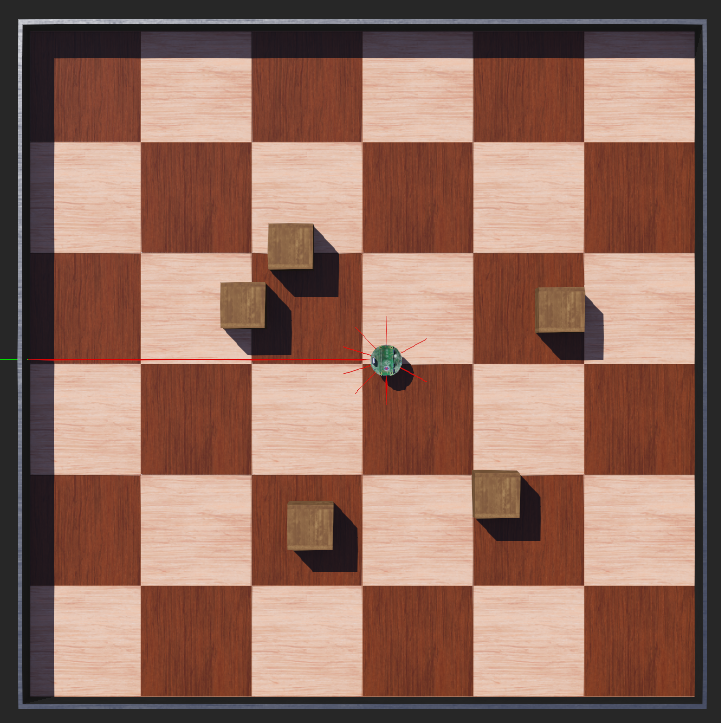
\includegraphics[width=0.65\textwidth]{./results/figures/map_epuck_vs_khepera.png}
    \caption{Map used to compare the behavior of e-puck2 and Khepera IV with the same \ac{ros2} controller}
    \label{fig:results:map_epuck_vs_khepera}
\end{figure}

\subsection{Performance Comparison in Mapping}

In Figure \ref{fig:results:epuck2_vs_khepera4_map_results} we can notice that both robots managed to map the environment.

\begin{figure}[H]
    \centering
    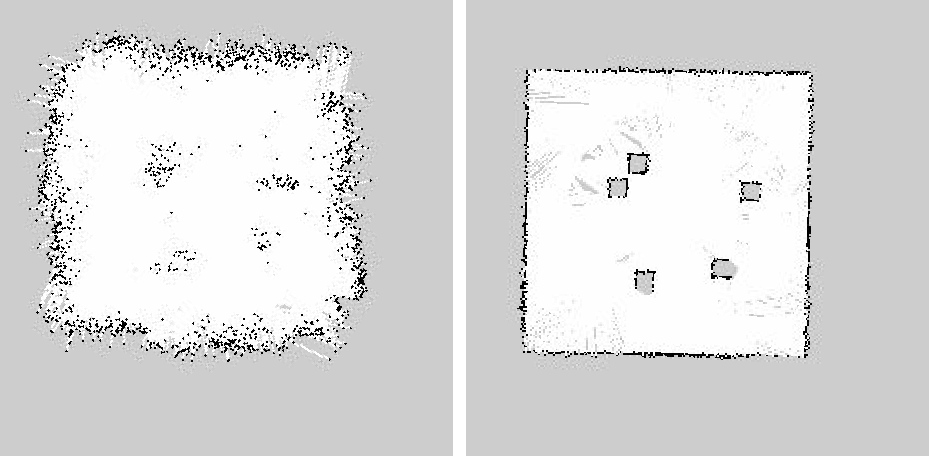
\includegraphics[width=\textwidth]{./results/figures/epuck2_vs_khepera4_map_results}
    \caption{Map produced by Khepera IV (left) and e-puck2 (right)}
    \label{fig:results:epuck2_vs_khepera4_map_results}
\end{figure}

It proofs it is possible to use different robots with same \ac{ros2} controller.
However, \ac{tof} sensor available on the e-puck2 robot provides visibly better performance in mapping compared to Khepera IV with ultrasonic sensors.
The main reason in poor map quality of produced by Khepera IV robot is high noise in ultrasonic sensors.

\subsection{Performance Comparison in Navigation}

Navigation analysis is done in same way as in Section \ref{results:subsec:phy_navigation}, but with a different map (see Figure \ref{fig:results:nav_goal}).

\begin{figure}[H]
    \centering
    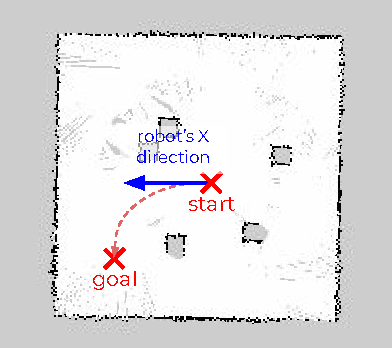
\includegraphics[width=0.5\textwidth]{./results/figures/nav_goal}
    \caption{Navigation goal on the map}
    \label{fig:results:nav_goal}
\end{figure}

Similarly to the previous navigation comparison the result is shown in Figure \ref{fig:results:simulated_navigation_comparison}.

\begin{figure}[H]
    \centering
    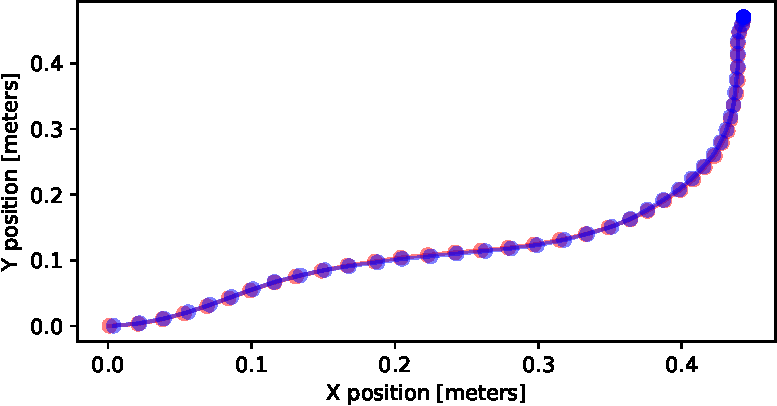
\includegraphics[width=\textwidth]{./results/figures/simulated_navigation_comparison}
    \caption{Path chosen by e-puck2 (red) and path chosen by Khepera IV (blue)}
    \label{fig:results:simulated_navigation_comparison}
\end{figure}

\section{Benefits of Generalized \ac{ros2} Interface for Webots}

Generalized \ac{ros2} driver on e-puck2 robot has produces the same \ac{ros2} interface as a specific \ac{ros2} driver given in Chapter \ref{chap:simulation}.
Therefore, in this section, a brief overview on using the generalized \ac{ros2} driver with other robots will be given.

\subsection{Khepera IV Driver Analysis}

In the first figure (Figure \ref{fig:results:khepera4_transforms}), a result of URDF export is shown.
The figure shows a different coordinate frames exported with the new Webots \ac{api} function.

\begin{figure}[H]
    \centering
    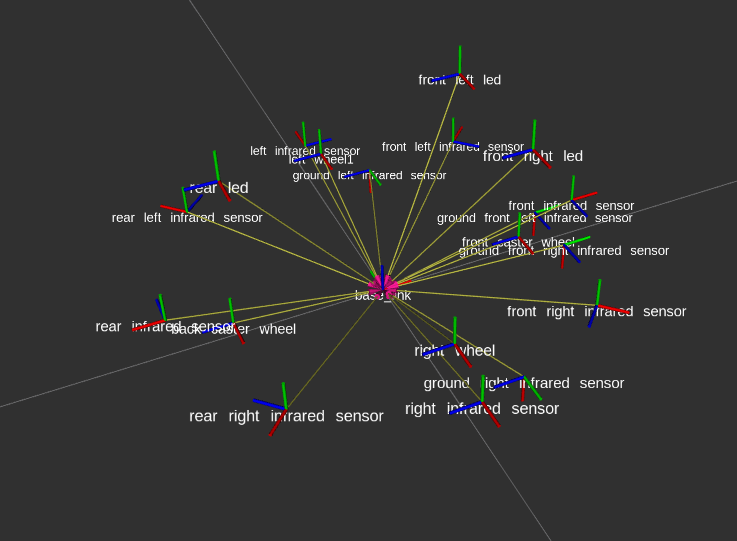
\includegraphics[width=1\textwidth]{./results/figures/khepera4_transforms}
    \caption{Coordinate frames generated by \ac{urdf} exporter}
    \label{fig:results:khepera4_transforms}
\end{figure}

Another aspect is \ac{ros2} \ac{api} available in Table \ref{tab:result:khepera4_api}.

\begin{table}[H]
    \begin{adjustwidth}{-1.5in}{-1.5in}
    \centering
    \begin{tabular}{|l|l|l|}
        \hline
        \textbf{Topic name} & \textbf{Message type} & \textbf{Description} \\
        \hline
        /camera/camera\_info & sensor\_msgs/CameraInfo & Camera intrinsic parameters \\
        \hline
        /camera/image\_raw & sensor\_msgs/Image & Images from camera \\
        \hline
        /cmd\_vel & geometry\_msgs/Twist & Velocity control \\
        \hline
        /[position]\_infrared\_sensor (x12) & sensor\_msgs/Range & Infrared measurements \\
        \hline
        /[position]\_led (x3) & std\_msgs/Int32 & \ac{led} control \\
        \hline
        /[position]\_ultrasonic\_sensor (x5) & sensor\_msgs/Range & Ultrasonic measurements \\
        \hline
        /imu & sensor\_msgs/Imu & \ac{imu} measurements \\
        \hline
        /joint\_states & sensor\_msgs/JointState & Encoder measurements \\
        \hline
        /odom & nav\_msgs/Odometry & Odometry \\
        \hline
        /robot\_description & std\_msgs/String & \ac{urdf} as a string \\
        \hline
        /tf & tf2\_msgs/TFMessage & Dynamic transforms \\
        \hline
        /tf\_static & tf2\_msgs/TFMessage & Static transforms \\
        \hline
    \end{tabular}
    \caption{\ac{ros2} \ac{api} for Khepera IV robot}
    \label{tab:result:khepera4_api}
    \end{adjustwidth}
\end{table}

The table shows that the \ac{ros2} generalized driver managed to expose devices to the \ac{ros2} system.

\subsection{Going Beyond Khepera IV and E-puck2}

The \ac{ros2} generalized driver is tested on many robots.
In further text, a two examples will be given, TIAGo++ and TurtleBot3 Burger.

\subsubsection{TIAGo++ Robot}

TIAGo++ robot is designed by PAL Robotics to work in indoor environments.
Typically, the platform is used in research or light industry. 
To us, the robot is interesting because it has a lot of joints\footnote{A specific \ac{ros2} driver was already developed, but the universal driver presented in this thesis greatly extends its capabilities}.
Therefore, it is a good test for the \ac{urdf} exporter.

\begin{figure}[H]
\centering
\begin{subfigure}{1\textwidth}
  \centering
  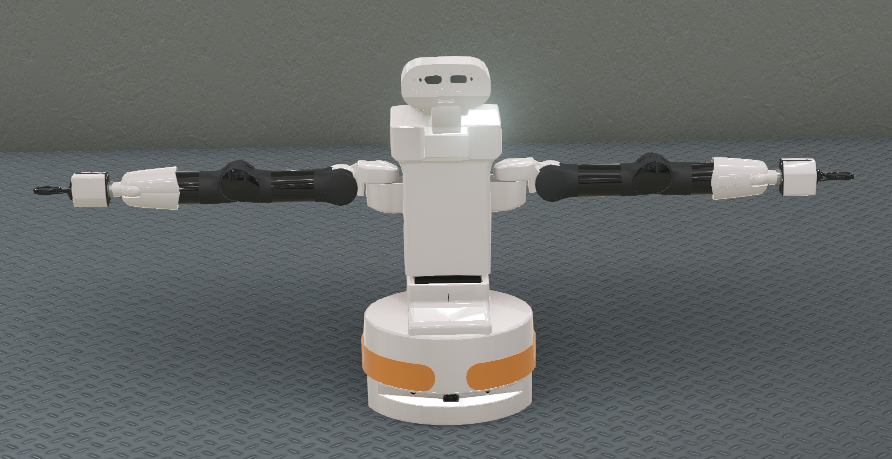
\includegraphics[width=\linewidth]{results/figures/tiago_webots.png}
  \caption{TIAGo++ model in Webots}
  \label{fig:results:map:webots}
\end{subfigure}
\begin{subfigure}{1\textwidth}
  \centering
  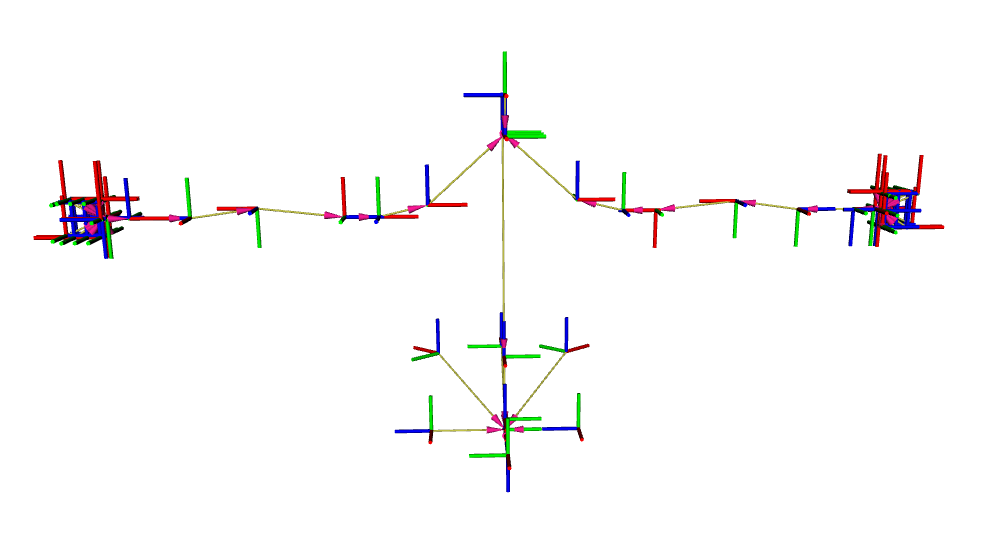
\includegraphics[width=\linewidth]{results/figures/tiago_frames.png}
  \caption{TIAGo++ frames in RViz2}
  \label{fig:results:tiago:frames}
\end{subfigure}
\caption{Result of \ac{urdf} exporter on TIAGo++ robot}
\label{fig:results:tiago}
\end{figure}

In Figure \ref{fig:results:tiago}, TIAGo++ model is shown in Webots as well its coordinates frames produced by the \ac{urdf} exporter.

\subsubsection{TurtleBot3 Burger Robot}

TurtleBot3 Burger is a small and affordable, often used by \ac{ros} team as a reference robot.
For us, it was important to verify whether the generalized \ac{ros2} driver is compatible with
the official \ac{ros2} package\footnote{The \ac{ros2} TurtleBot3 package is available at \url{https://github.com/ROBOTIS-GIT/turtlebot3}} provided by a team behind TurtleBot3 Burger.

\begin{figure}[H]
    \centering
    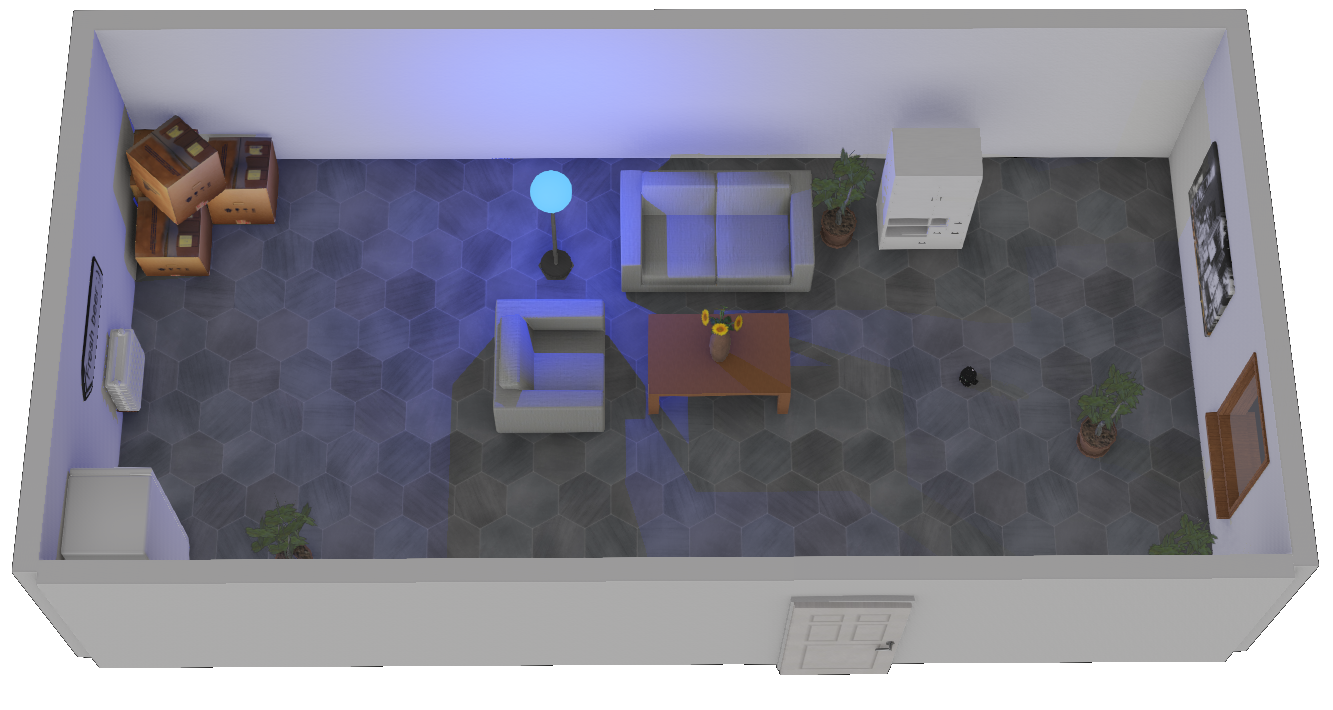
\includegraphics[width=\textwidth]{./results/figures/turtlebot_webots}
    \caption{Webots world used to verify TurtleBot3 Burger mapping and navigation capabilities}
    \label{fig:results:turtlebot_webots}
\end{figure}

In the figures bellow a RViz2 view for \ac{slam} (see Figure \ref{fig:results:turtlebot_mapping}) and navigation (see Figure \ref{fig:results:turtlebot_navigation}) are given.

\begin{figure}[H]
    \centering
    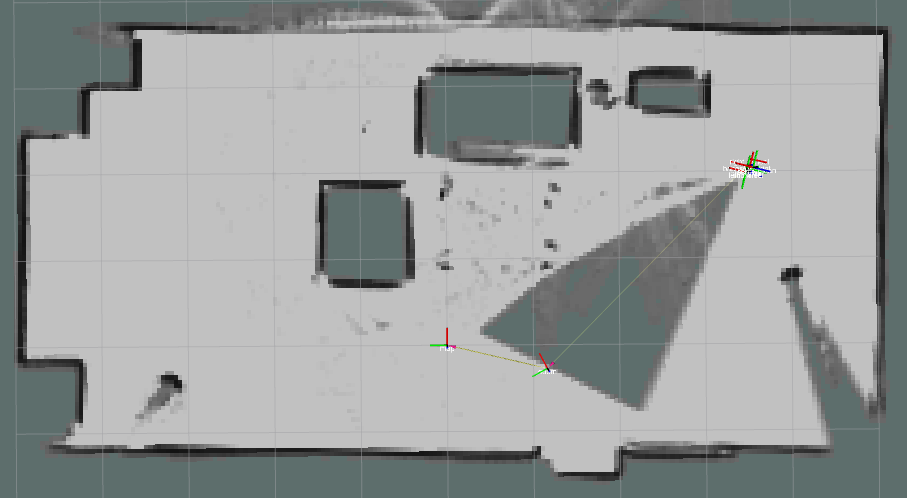
\includegraphics[width=\textwidth]{./results/figures/turtlebot_mapping}
    \caption[TurtleBot3 Burger mapping view in RViz2]{TurtleBot3 Burger mapping view in RViz2 (during the mapping process)}
    \label{fig:results:turtlebot_mapping}
\end{figure}

\begin{figure}[H]
    \centering
    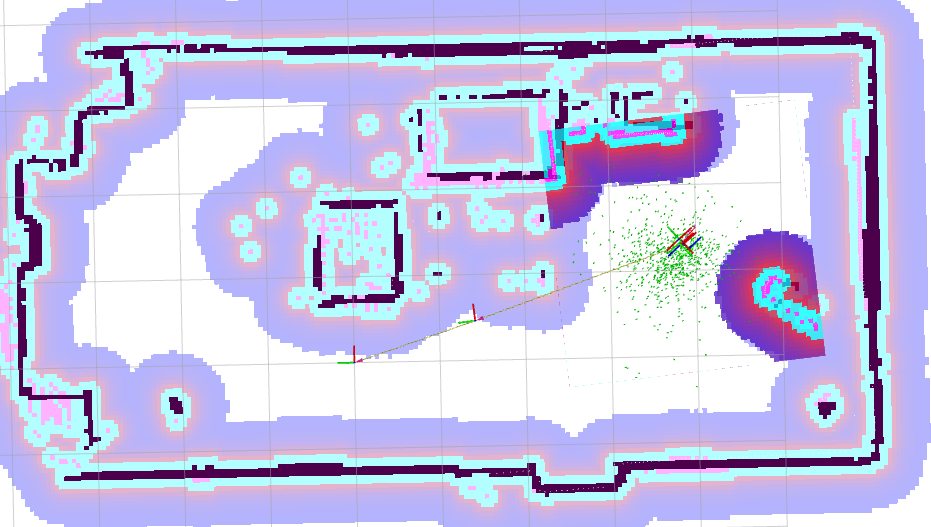
\includegraphics[width=\textwidth]{./results/figures/turtlebot_navigation}
    \caption{TurtleBot3 Burger navigation view in RViz2}
    \label{fig:results:turtlebot_navigation}
\end{figure}

The RViz2 views show that the TurtleBot3 package works as expected without any code modifications.
Overall, these experiments show that the generalized \ac{ros2} driver scales well to all tested scenarios.
